%!TEX root = ../var.tex

\begin{definition}
	Пусть $\Omega$ — пространство элементарных событий, и
$\mathfrak{A}$ — его $\sigma$-алгебра событий. Вероятностью называется функция множества
$P: \mathfrak{A}\rightarrow \mathbb{R}$, удовлетворяющая следующим аксиомам:

Акс.$\mathcal{P}1$ (\textit{неотрицательность вероятности}). Для любого события $A\in\mathfrak{A}$ выполнено равенство $P(A)\geqslant 0$.

Акс.$\mathcal{P}2$ (\textit{нормированность вероятности}). $P(\Omega)=1$ 

Акс.$\mathcal{P}3$ (\textit{счётная аддитивность вероятности как функции множества}).
\end{definition}
Для любого счётного набора попарно несовместных событий \newline $A_1,A_2,\dots\in 
\mathfrak{A}$
имеет место равенство
\begin{equation}
	P\left(\bigcup_{n=1}^{\infty}A_n \right)=\sum^{\infty}_{n=1}P(A_n) \notag
\end{equation}
В частности, эта аксиома справедлива и для конечного набора попарно несов
местных событий.
Акс. $\mathcal{P}1$ (непрерывность вероятности). Для любой убывающей последовательности событий $A_1 \supset A_2 \supset\dots\supset A_n \supset \dots$ из $\sigma$-алгебры $\mathfrak{A}$ такой, что $\bigcap_{n=1}^{\infty}A_n=\noo$,
выполняется равенство
\begin{equation}
	\lim\limits_{n\to\infty}P(A_n)=0 \notag
\end{equation}
\begin{definition}
	Тройка $(\Omega,\mathfrak(A),P)$ называется \textit{вероятностным пространством}.
\end{definition}
Докажем теперь основные свойства вероятности пп. \ref{lemma:3.3} – \ref{t:3.12}.
\begin{lemma}
	\label{lemma:3.3}
	Если событие A влечёт событие B, т.е $A\subseteq B$, то $P(B\ssm A)=P(B)-P(A)$
\end{lemma}

\begin{proof}
	Т.к. $B=A\cup(B\ssm A)$,  и события A и $B\ssm A $ несовместны, то по аксиоме $\mathfrak{P}$ имеем $P(B)=P(A)+P(B\ssm A)$, что и требовалось доказать.
\end{proof}
\begin{figure}[H]
	\centering
	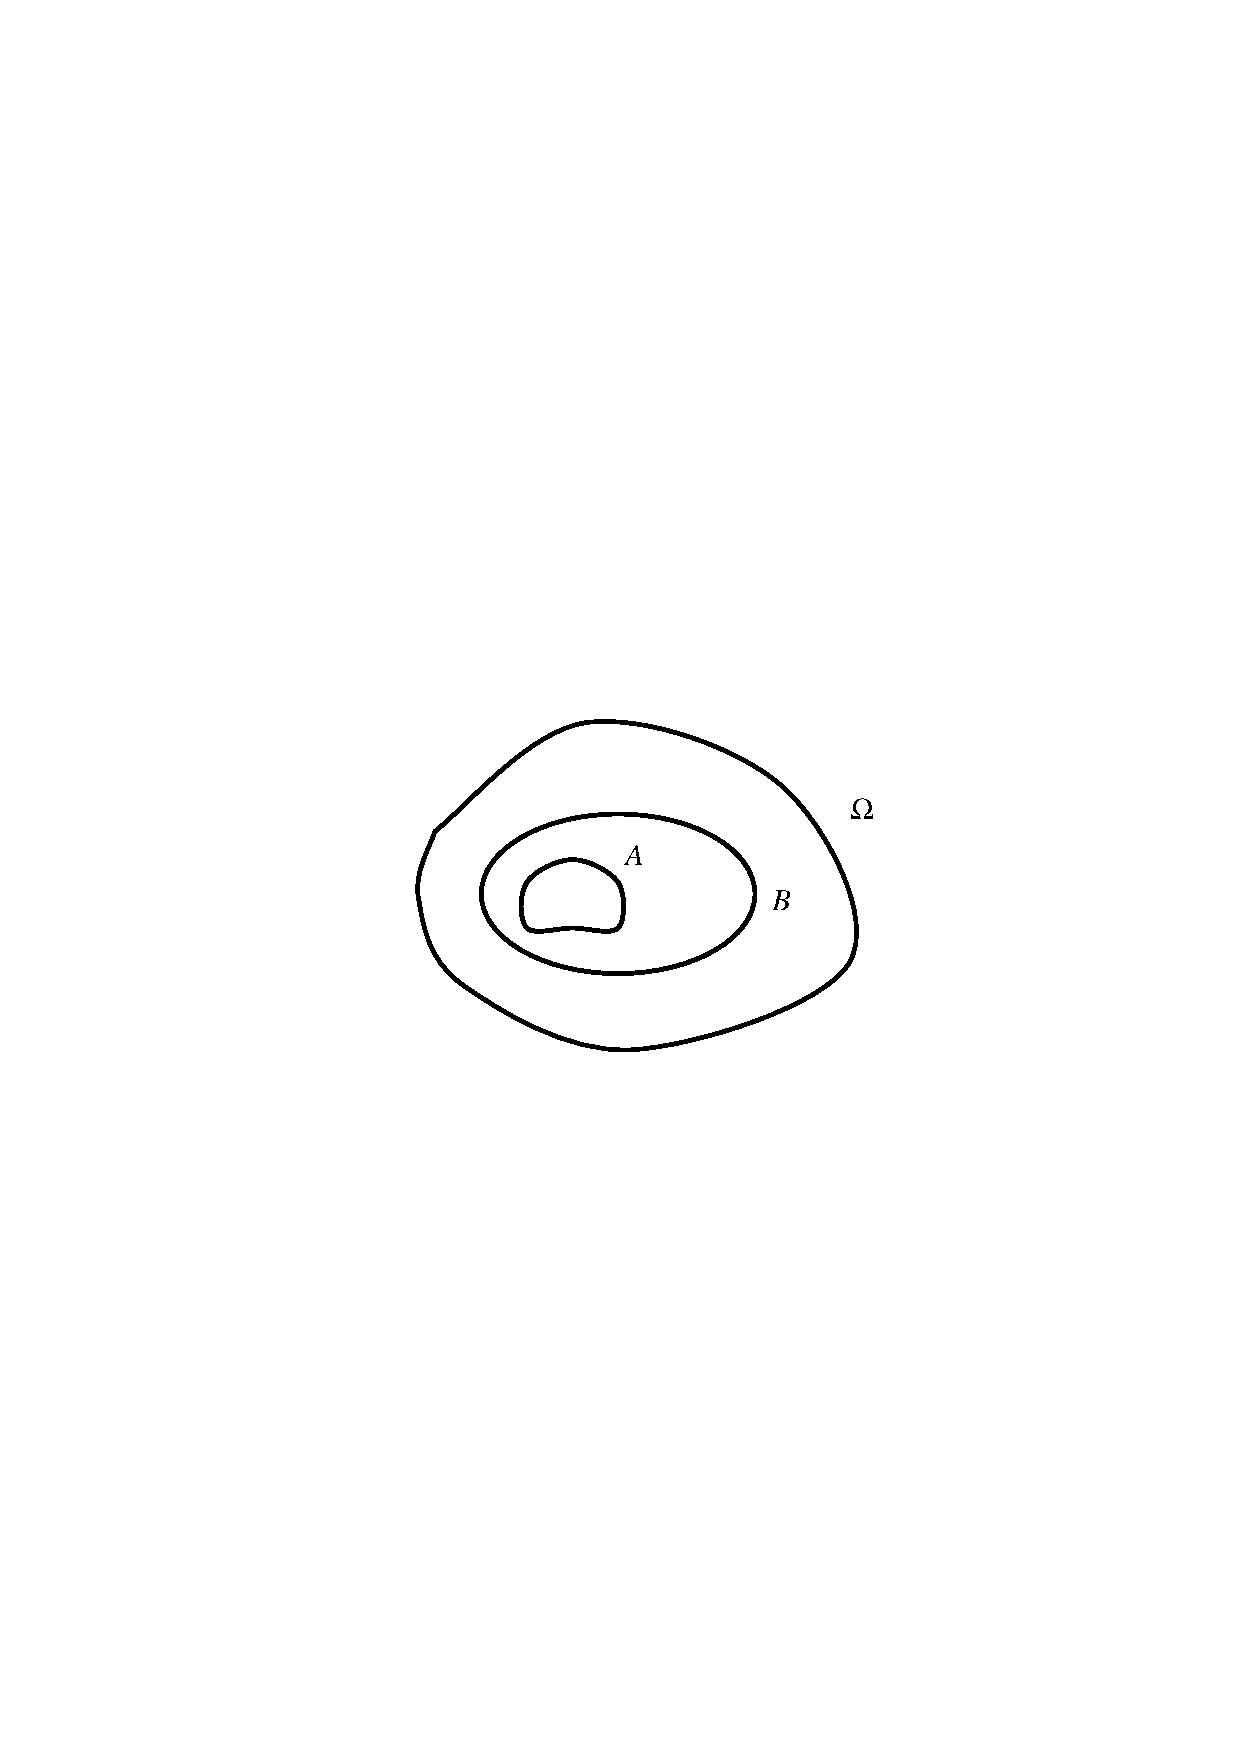
\includegraphics[width=0.5\textwidth]{pic/pic2.pdf}
	\caption{Если $A\subseteq B$, то $P(B\ssm A=P(B)-P(A))$.}
	\label{pic:2}
\end{figure}

\begin{consq}
	\label{consq:1}
	Если $A\subseteq B$, то $P(A)\geqslant P(B)$. 
\end{consq}

\begin{lemma}
	$P(\noo)=0$.
\end{lemma}
\begin{proof}
	$P(\noo)=P(\Omega\ssm\Omega)=P(\Omega)=P(\Omega)=1-1=0$
\end{proof}

\begin{lemma}
	Для любого события $A\in\mathfrak{A}$ выполнено неравенство
	\begin{equation*}
		0\leqslant P(A)\leqslant 1
	\end{equation*}
\end{lemma}
\begin{proof}
	Т.к. $\O\subseteq A\subseteq\Omega$, то из след. \ref{consq:1} следует утверждение леммы. 
\end{proof}

\begin{lemma}
	Для любого события $A\in\mathfrak(A)$ имеем $P(\bar{A})=1-P(A)$
\end{lemma}

\begin{proof}
	$P(\bar{A})=P(\Omega\ssm A)=P(\Omega-P(A)=1-P(A)$
\end{proof}

\begin{lemma}
	\label{lemma:3.8}
	Для любых событий $A,B\in\mathfrak(A)$ выполнено равенство 
\begin{equation*}
	P(A\cup B)=P(A)+P(B)-P(A\cap B).
\end{equation*}
	
\end{lemma}
\begin{proof}
	Т.к. $A\cup B = A \cup(B \ssm (A \cup B))$, и события $A$ и
$B \ssm (A \cup B)$ несовместны, то применяя сначала Акс. $\mathcal{P}3$, а затем лемму \ref{lemma:3.3}
получим $P(A\cup B) = P(A) + P(B \ssm (A\cup B)) = P(A) + P(B) − P(A \cup B)$.
\end{proof}
\begin{consq}
	Для любых событий $A,B\in\mathfrak{A}$ выполнено равенство 
	\begin{equation*}
		P(A\cup B)\geqslant P(A)+P(B).
	\end{equation*}
\end{consq}

\begin{consq}
	Если события A и B несовместны, т.е $A\cap B=\O$, то 
\begin{equation*}
		P(A\cup B)\leqslant P(A)+P(B).
\end{equation*}
\end{consq}

\begin{proof}
	По лемме \ref{lemma:3.8} имеем $P(A\cup B)=P(A)+P(B)-P(A\cap B)=P(A)+P(B)-P(\noo)=P(A)+P(B)$.
\end{proof}

\begin{consq}
	$P(A_1\cup\dots\cup A_n)\leqslant\sum\limits^n_{i=1}P(A_i)$.
\end{consq}	
\begin{theorem}
\label{t:3.12}
\begin{gather*}
	P(A_1\cup A_2\cup\dots A_n)
	=\sum\limits_{i=1}^n P(A_i)
	-\sum\limits_{1\leqslant i<j	\leqslant n} P(A_i\cap A_j)\\
	+ \sum\limits_{1\leqslant i<j<m\leqslant n}P(A_i\cap A_j \cap A_m)-
	\dots
	+(-1)^{n-1}P(A_1\cap A_2\cap\dots\cap A_n).
\end{gather*}
\begin{proof}
	Применяя метод математической индукции и лемму \ref{lemma:3.8}
получим требуемый результат.
\end{proof}
\end{theorem}
